\chapter{التحكم في دورة الخلية والموت الخلوي المبرمج}\label{ch:b3:cell-cycle-apoptosis}

نحو مئة مليار خلية من جسمك ستموت اليوم، عن قصد،
وستولد مئة مليار لتحل محلها؛ فبطانة
أمعائك تتجدد كل خمسة أيام، وكرياتك الحمر كل أربعة أشهر.
والشرغوف يفقد ذيله بلا نزف؛ والغشاء بين أصابع الجنين
البشري يختفي في الأسبوع الثامن؛ ونصف العصبونات المصنوعة
في دماغ تُقتل قبل الولادة. وكل واحد من هذه الموتات
تنفذه الخلية نفسها، على برنامج، وكل واحدة من
الولادات يرخّص لها نظام تحكم يقرر، عند نقطتين أو ثلاث
في الدورة، هل يجوز للخلية أن تمضي. والبرنامجان
--- الانقسام والانتحار --- موضوع هذا الفصل. وقد
حُلّا في الخميرة، وبيوض الضفادع، وقنافذ البحر، ودودة فيها بالضبط
$1090$ خلية جسدية يموت منها بالضبط $131$، ثم تبيّن أنهما
هما نفسهما في البشر، حيث إخفاقهما سرطان من جهة و
تنكّس من أخرى.

\section{محرّك الدورة}

\begin{definition}[السيكلينات والكينازات المعتمدة على السيكلين]\label{def:b3:cell-cycle-apoptosis:cdk}
\index{سيكلين}\index{كيناز معتمد على السيكلين}\index{معقّد تعزيز الطور الانفصالي}\index{دورة الخلية}
دورة الخلية --- G1، وS (التضاعف)، وG2، وM (الانقسام الفتيلي) --- يقودها
طقم من كينازات البروتين، هي \emph{الكينازات المعتمدة على السيكلين}
(CDK)، ووحداتها الحفّازة حاضرة طوال الدورة لكنها
لا تنشط إلا حين ترتبط بوحدة \emph{سيكلين}، وهو وحدة تنظيمية يرتفع
تركيزها ويهبط بترتيب ثابت: فالسيكلين D مع Cdk4/6 في
G1 استجابةً لعوامل النمو، والسيكلين E مع Cdk2 عند انتقال
G1/S، والسيكلين A مع Cdk2 خلال S، والسيكلين B مع Cdk1 عند
الدخول في الانقسام الفتيلي. ويفسفر كل زوج سيكلين--CDK بروتينات
طوره --- مناشئ التضاعف، واللامينات، والمكثِّفات، وإنزيمات
تجميع المغزل --- ويُطفأ كل منها بهدم
سيكلينه: إذ توسم ليغازات اليوبيكويتين (SCF في G1/S، و\emph{معقّد
تعزيز الطور الانفصالي}، APC/C، في الانقسام الفتيلي) السيكلينات للبروتيازوم. و
نشاط Cdk1 تحكمه فوق ذلك فسفرة مثبطة يضعها
الكيناز Wee1 ويزيلها الفوسفاتاز Cdc25، وبروتينات
مثبطة صغيرة (p21 وp27 وp16) ترتبط بالمعقّدات. و
الدورة إذن تسلسل منتظم من موجات الكينازات، تنتهي كل موجة
بتحلل ما أنتجها.
\end{definition}

\begin{proof}[شواهد]
تلاقت ثلاثة خطوط. فعزل هارتويل (في سبعينيات القرن العشرين) طافرات
\emph{cdc} حساسة للحرارة من خميرة التبرعم، كل منها متوقف عند طور
بحجم برعم مميز، وحدد \emph{البداية}، وهي النقطة في G1 التي بعدها
تلتزم الخلية بدورة. ووجد نيرس (في الثمانينيات) في خميرة
الانشطار أن \emph{cdc2} يتحكم في توقيت الانقسام الفتيلي وأن
المورّثة البشرية، إذا وُضعت في الخميرة، أنقذت الطافر: فالكيناز هو
Cdk1، محفوظ من الخميرة إلى الإنسان. ووجد هانت (1983) في بيوض قنفذ
البحر بروتينًا يتراكم خلال كل دورة ويُهدم
فجأةً عند كل انقسام، وسماه \omterm{def:b3:cell-cycle-apoptosis:cdk}{سيكلين}. وكانت بيضة الضفدع
قد أعطت في هذه الأثناء ``عامل تعزيز النضج'' الذي يدفع أي
نواة إلى الانقسام الفتيلي؛ وتبيّن أنه \omterm{def:b3:cell-cycle-apoptosis:cdk}{السيكلين} B مرتبطًا بكيناز Cdk1. وكان راو وجونسون
(1970) قد بيّنا بدمج الخلايا أن خلية في الطور S تدفع نواةً في
G1 إلى التضاعف، بينما تنتظر نواة في G2 --- فالهيولى
تحمل الإشارة، والنواة المتضاعفة لا يمكن حملها على أن
تتضاعف ثانيةً.
\end{proof}

\begin{omfigure}
\begin{tikzpicture}[every node/.style={font=\scriptsize}, >=stealth]
  % cycle circle with phases
  \draw[very thick, omDef!50] (0,0) circle (2.2);
  \foreach \a/\b/\col/\lab/\r in {90/200/omDef!25/G1/1.55, 200/270/omProp!30/S/1.55, 270/315/omMeth!30/G2/1.55, 315/450/omThm!30/M/1.55} {
    \fill[\col] (0,0) -- (\a:2.2) arc[start angle=\a, end angle=\b, radius=2.2] -- cycle;
    \node[font=\small\bfseries] at ({(\a+\b)/2}:\r) {\lab};
  }
  \fill[white] (0,0) circle (1.0);
  \draw[very thick, omDef!50] (0,0) circle (2.2);
  % cyclin-CDK labels around
  \node[left, align=right] at (-2.4,1.2) {سيكلين D--Cdk4/6\\عوامل النمو، إطفاء Rb};
  \node[left, align=right] at (-2.4,-1.0) {سيكلين E--Cdk2\\إطلاق المناشئ};
  \node[anchor=north east, align=right] at (-1.3,-2.2) {سيكلين A--Cdk2\\التضاعف};
  \node[right, align=left] at (2.4,-1.0) {سيكلين B--Cdk1\\الدخول في الانقسام الفتيلي};
  \node[right, align=left] at (2.4,1.3) {APC/C يهدم السيكلين B\\والسكيورين: الطور الانفصالي، والخروج};
  % checkpoints as bars
  \foreach \a in {160,270,20} \draw[very thick, omThm] (\a:1.95) -- (\a:2.45);
  \node[align=center, anchor=south east] at (-1.2,2.35) {نقطة التقييد:\\أعوامل نمو؟};
  \node[align=left, anchor=west] at (2.55,0.35) {نقطة تفتيش المغزل:\\أكل القسيمات المركزية مرتبطة؟};
  \node[align=center, anchor=north] at (1.5,-2.55) {نقطة تفتيش G2/M:\\أDNA سليم؟};
  \draw[->, thick] (0,0) ++(60:1.25) arc[start angle=60, end angle=30, radius=1.25];
\end{tikzpicture}

{\small الدورة متتاليةً من موجات السيكلين--CDK، تنهي كلًا منها
هدمُ سيكلينها، مع نقاط التفتيش الثلاث (الأشرطة الحمراء) التي
تسأل عندها الخلية هل تمضي.}
\end{omfigure}

\begin{theorem}[مفتاح ومكبح مؤجَّل يصنعان مذبذبًا]\label{thm:b3:cell-cycle-apoptosis:oscillator}
\index{مذبذب استرخائي}\index{ثنائية الاستقرار!في دورة الخلية}\index{تخلّف}
ليكن $A$ نشاط \omterm{def:b3:cell-cycle-apoptosis:cdk}{السيكلين} B--Cdk1 و$C$ كمية \omterm{def:b3:cell-cycle-apoptosis:cdk}{السيكلين}
B. ولنفترض (1) أنه من أجل $C$ ثابتة، تسترخي $A$ سريعًا إلى حالة مستقرة
تتوقف على $C$ عبر تغذية راجعة موجبة (إذ ينشّط Cdk1 الفعال
منشّطه Cdc25 ويثبط مثبطه Wee1)، بحيث يكون
منحني الحالة المستقرة $A^{*}(C)$ على شكل حرف S: فمن أجل $C$ بين
عتبتين $C_{1} < C_{2}$ توجد حالة منخفضة وأخرى مرتفعة معًا، ويبقى
النظام على الفرع الذي هو عليه (وهو \emph{التخلّف})؛ و(2) أن $C$
تتغير ببطء، فتُركَّب بمعدل ثابت $k_{s}$ وتُحلَّل بمعدل
$k_{d}A\,C$ عبر APC/C، الذي يشغّله Cdk1 الفعال
بعد تأخير. عندئذٍ لا تكون للنظام حالة مستقرة ثابتة وينفذ
\emph{تذبذبًا استرخائيًا}: إذ تتراكم $C$ على الفرع المنخفض حتى
تتجاوز $C_{2}$، فتقفز $A$ إلى الفرع المرتفع (وهو الدخول في الانقسام)،
ويسبق التحللُ التركيبَ وتهبط $C$ حتى تتجاوز $C_{1}$، فتنهار $A$
إلى الفرع المنخفض (وهو الخروج من الانقسام)، وتتكرر الدورة. و
يحدد الدورَ أساسًا المتغيرُ البطيء: أي نحو $C_{2}/k_{s}$ في
الصعود، زائدًا زمن التحلل من $C_{2}$ إلى $C_{1}$.
\end{theorem}
\begin{proof}[برهان جزئي]
الحالة المستقرة للزوج تقتضي $\mathrm{d}C/\mathrm{d}t = 0$،
أي $k_{s} = k_{d}A^{*}(C)\,C$، عند نقطة على المنحني الذي على شكل S.
وعلى الفرع المنخفض تكون $A^{*}$ صغيرة، فتكون $k_{d}A^{*}C < k_{s}$ من أجل $C$ حتى
$C_{2}$: فيرتفع \omterm{def:b3:cell-cycle-apoptosis:cdk}{السيكلين}، ويُحمل النظام خارج نهاية
الفرع. وعلى الفرع المرتفع تكون $A^{*}$ كبيرة، فتكون $k_{d}A^{*}C > k_{s}$ من أجل
$C$ نزولًا إلى $C_{1}$: فيهبط \omterm{def:b3:cell-cycle-apoptosis:cdk}{السيكلين}، ويُحمل النظام خارج تلك
النهاية. والحالة المستقرة المرشحة الوحيدة كانت لتقع على الفرع
الأوسط غير المستقر، والنقطة هناك طاردة؛ فلا توجد إذن حالة مستقرة
ثابتة، ويتذبذب المسار المحصور في الفرعين المستقرين
وفي القفزتين بينهما. والزمن على الفرع المنخفض هو
$\int \mathrm{d}C/(k_{s} - k_{d}A^{*}C) \approx C_{2}/k_{s}$ حين تكون
$A^{*}$ صغيرة، والزمن على الفرع المرتفع هو الزمن الأقصر
لتحلل $C_{2} - C_{1}$ بمعدل $k_{d}A^{*}_{\text{مرتفع}}C$. أما
وجود المنحني الذي على شكل S من تغذية Cdc25/Wee1 الراجعة فمسلَّم
به هنا؛ وهو ثنائية الاستقرار نفسها في المورّثة ذاتية التنشيط
في كتاب السنة~الثانية، مع كون المتغير السريع كينازًا هنا والبطيء
سيكلينه.
\end{proof}

\begin{omfigure}
\begin{tikzpicture}
\begin{axis}[
  width=6.6cm, height=5.6cm,
  axis lines=left,
  xmin=0, xmax=1.4, ymin=0, ymax=1.1,
  xlabel={السيكلين B، $C$}, ylabel={نشاط Cdk1، $A$},
  xlabel style={font=\small, at={(axis description cs:0.5,-0.12)}, anchor=north}, ylabel style={font=\small},
  tick label style={font=\scriptsize}, xtick={0.4,1.0}, xticklabels={$C_{1}$,$C_{2}$}, ytick=\empty,
  clip=false,
]
% S-shaped nullcline: two stable branches and a dashed unstable one
\addplot[very thick, omDef, smooth] coordinates {(0,0.02) (0.5,0.04) (0.9,0.07) (1.0,0.1)};
\addplot[very thick, omDef, dashed, smooth] coordinates {(1.0,0.1) (0.85,0.3) (0.7,0.5) (0.55,0.7) (0.4,0.9)};
\addplot[very thick, omDef, smooth] coordinates {(0.4,0.9) (0.6,0.94) (1.0,0.97) (1.4,0.98)};
\draw[->, very thick, omThm] (axis cs:0.05,0.15) -- (axis cs:0.98,0.15);
\draw[->, very thick, omThm] (axis cs:1.04,0.18) -- (axis cs:1.04,0.82);
\draw[->, very thick, omThm] (axis cs:0.98,0.84) -- (axis cs:0.42,0.84);
\draw[->, very thick, omThm] (axis cs:0.36,0.82) -- (axis cs:0.36,0.18);
\node[font=\scriptsize, omThm, anchor=south west] at (axis cs:0.36,0.24) {يتراكم السيكلين};
\node[font=\scriptsize, omThm, anchor=west] at (axis cs:1.07,0.5) {دخول};
\node[font=\scriptsize, omThm, anchor=south] at (axis cs:0.7,1.0) {APC/C يحلل السيكلين (الانقسام الفتيلي)};
\node[font=\scriptsize, omThm, anchor=east] at (axis cs:0.33,0.5) {خروج};
\node[font=\scriptsize, omDef, anchor=north east] at (axis cs:1.38,0.95) {$A^{*}(C)$};
\end{axis}
\begin{axis}[
  at={(7.6cm,0)}, anchor=south west,
  width=6.6cm, height=5.6cm,
  axis lines=left,
  xmin=0, xmax=3, ymin=0, ymax=1.2,
  xlabel={الزمن (دورات)}, ylabel={},
  xlabel style={font=\small, at={(axis description cs:0.5,-0.12)}, anchor=north},
  tick label style={font=\scriptsize}, xtick={0,1,2,3}, ytick=\empty,
  clip=false,
]
\addplot[very thick, omDef] coordinates {(0,0.4) (0.8,1.0) (0.95,0.4) (1.75,1.0) (1.9,0.4) (2.7,1.0) (2.85,0.4) (3,0.5)};
\addplot[very thick, omThm] coordinates {(0,0.05) (0.8,0.05) (0.8,0.95) (0.95,0.95) (0.95,0.05) (1.75,0.05) (1.75,0.95) (1.9,0.95) (1.9,0.05) (2.7,0.05) (2.7,0.95) (2.85,0.95) (2.85,0.05) (3,0.05)};
\node[font=\scriptsize, omDef, anchor=south west] at (axis cs:1.0,0.1) {السيكلين B};
\node[font=\scriptsize, omThm, anchor=south west] at (axis cs:1.0,1.0) {نشاط Cdk1};
\end{axis}
\end{tikzpicture}

{\small يسارًا: مستوي طور المذبذب. المنحني الذي على شكل S هو
الحالة المستقرة السريعة لكيناز Cdk1 عند كل مستوى من \omterm{def:b3:cell-cycle-apoptosis:cdk}{السيكلين}؛ والعروة الحمراء
هي الدورة --- تراكم بطيء على الفرع المنخفض، وقفزة عند
$C_{2}$، وتحلل سريع على الفرع المرتفع، وقفزة عودة عند
$C_{1}$. يمينًا: السير الزمني الناتج، سنّ منشار من \omterm{def:b3:cell-cycle-apoptosis:cdk}{السيكلين} وموجة
مربعة من الكيناز.}
\end{omfigure}

\begin{example}[لماذا تكون بيضة الضفدع ساعة]\label{ex:b3:cell-cycle-apoptosis:frog}
بيضة ضفدع ملقحة تنقسم اثنتي عشرة مرة في ست ساعات بلا
نمو ولا استنساخ ولا نقاط تفتيش، على فترات قدرها
\qty{30}{min}: فهي مذبذب المبرهنة يعمل عاريًا، ومستخلص
من هيولاها في أنبوب اختبار يظل يدور، \omterm{def:b3:cell-cycle-apoptosis:cdk}{والسيكلين} يرتفع
ويهبط، بلا شيء ينقسم. وإضافة \omterm{def:b3:cell-cycle-apoptosis:cdk}{سيكلين} B غير قابل للتحلل
تحبس المستخلص في الانقسام الفتيلي، إذ لا تستطيع $C$ أن تهبط دون $C_{1}$؛
وحجب تركيب \omterm{def:b3:cell-cycle-apoptosis:cdk}{السيكلين} يحبسه في الطور البيني. وفي الخلية الجسدية
يُغلَّف المحرّك نفسه بضوابط القسم التالي، التي تمسكه
عند العتبات حتى تُستوفى الشروط، فيصير الدور
يومًا لا نصف ساعة ويمكن أن يطول بلا حد.
\end{example}

\section{نقاط التفتيش}

\begin{definition}[نقاط التفتيش]\label{def:b3:cell-cycle-apoptosis:checkpoints}
\index{نقطة تفتيش}\index{نقطة التقييد}\index{نقطة تفتيش تجميع المغزل}\index{ترخيص التضاعف}
\emph{نقطة التفتيش} ضابط يوقف الدورة عند انتقال
حتى يتحقق شرط، بالعمل على المحرّك --- بتثبيط
كيناز CDK أو ليغاز يوبيكويتين. وثلاث منها أهمها. \emph{نقطة
التقييد} في أواخر G1 (وهي البداية في الخميرة): فلا تمضي الخلية إلا إذا سمحت
عواملُ النمو والمغذيات والحجم؛ وبعدها تكمل الدورة
من دونها. و\emph{نقطة تفتيش G2/M}: إذ إن DNA المتأذي أو غير المتضاعف،
الذي يشير إليه كينازا \omterm{def:b3:dna-repair:ddr}{ATM}/ATR في \cref{ch:b3:dna-repair}، يُبقي
Cdc25 مثبطًا فيُبقي Cdk1 مفسفرًا خاملًا. و
\emph{نقطة تفتيش تجميع المغزل}: فالقسيم المركزي الواحد غير المرتبط
بالأنيبيبات الدقيقة ينتج مثبطًا قابلًا للانتشار (وهو Mad2 مرتبطًا ببروتين Cdc20)
يُبقي APC/C مطفأً، فينتظر الطور الانفصالي آخر
صبغي. وثمة ضابط رابع لا خطوة انتظار فيه لكنه صارم
بالقدر نفسه: \emph{ترخيص التضاعف}. فتُحمَّل المناشئ بهليكاز
MCM في G1 وحده، حين يكون نشاط CDK منخفضًا، وتُهدم عوامل التحميل
أو تُثبَّط متى بدأ الطور S، فيُطلَق كل منشأ
مرة واحدة لا غير في الدورة --- وهو سبب عجز نواة G2 في دمج راو
وجونسون عن أن تُحمل على التضاعف.
\end{definition}

\begin{proposition}[نقطة التقييد مفتاح]\label{prop:b3:cell-cycle-apoptosis:rb}
\index{بروتين الورم الأرومي الشبكي}\index{E2F}
في أوائل G1 يكون عامل الاستنساخ \emph{E2F}، الذي يقود مورّثات
الطور S (\omterm{def:b3:cell-cycle-apoptosis:cdk}{السيكلين} E، \omterm{def:b3:cell-cycle-apoptosis:cdk}{والسيكلين} A، وإنزيمات التضاعف)، ممسكًا
خاملًا في قبضة \emph{\omterm{prop:b3:cell-cycle-apoptosis:rb}{بروتين الورم الأرومي الشبكي}} Rb. وتحرّض عوامل النمو
\omterm{def:b3:cell-cycle-apoptosis:cdk}{السيكلين} D، فيبدأ \omterm{def:b3:cell-cycle-apoptosis:cdk}{السيكلين} D--Cdk4/6 بفسفرة Rb، فيحرر
قليلًا من E2F؛ ثم يحرّض E2F \omterm{def:b3:cell-cycle-apoptosis:cdk}{السيكلين} E، ويفسفر \omterm{def:b3:cell-cycle-apoptosis:cdk}{السيكلين} E--Cdk2
بروتين Rb أكثر بكثير --- وهي تغذية راجعة موجبة تكمل نفسها متى تجاوزت عتبةً،
من غير حاجة إلى مزيد من عامل النمو. وتكون الخلية قد اجتازت
\omterm{def:b3:cell-cycle-apoptosis:checkpoints}{نقطة التقييد}؛ ويحرّض E2F مورّثته هو أيضًا. وفقدُ Rb، أو
فقدُ مثبط Cdk4/6 وهو p16، أو تضخيم \omterm{def:b3:cell-cycle-apoptosis:cdk}{السيكلين} D، يزيل
الحاجة إلى عامل النمو أصلًا، وكل منها شائع في
السرطان (\cref{ch:b3:cancer-biology})؛ والأدوية التي تثبط Cdk4/6 تُستعمل اليوم
ضد سرطانات الثدي التي تعتمد على هذا المفتاح.
\end{proposition}

\begin{omfigure}
\begin{tikzpicture}[every node/.style={font=\scriptsize}, >=stealth]
  \node[draw, thick, rounded corners, fill=omProp!25, minimum width=2.2cm] (gf) at (0,2.2) {عوامل النمو};
  \node[draw, thick, rounded corners, fill=omDef!20, minimum width=2.4cm] (cd) at (0,1.0) {سيكلين D--Cdk4/6};
  \node[draw, thick, rounded corners, fill=omThm!20, minimum width=1.6cm] (rb) at (3.8,1.0) {Rb};
  \node[draw, thick, rounded corners, fill=omMeth!25, minimum width=1.6cm] (e2f) at (7.2,1.0) {E2F};
  \node[draw, thick, rounded corners, fill=omDef!20, minimum width=2.4cm] (ce) at (7.2,-0.6) {سيكلين E--Cdk2};
  \node[draw, thick, rounded corners, fill=gray!15, align=center, minimum width=2.6cm] (s) at (10.8,1.0) {مورّثات الطور S:\\سيكلين A، وMCM، \dots};
  \draw[->, thick] (gf) -- (cd);
  \draw[-|, thick, omThm] (cd) -- (rb) node[midway, above, font=\tiny] {يفسفر};
  \draw[-|, thick, omThm] (rb) -- (e2f) node[midway, above, font=\tiny] {يمسكه خاملًا};
  \draw[->, thick] (e2f) -- (s);
  \draw[->, thick] (e2f) -- (ce) node[midway, right] {يحرّض};
  \draw[-|, thick, omThm] (ce.west) -- ++(-2.2,0) |- (rb.south) node[pos=0.25, below] {يفسفر Rb أكثر};
  \draw[->, thick, omMeth!70!black] (e2f.north) .. controls (6.0,2.2) and (6.8,2.2) .. (e2f.north east) node[pos=0.5, above] {يحرّض مورّثته هو};
  \node[draw, thick, rounded corners, fill=omThm!10] (p16) at (0,-0.6) {p16}; \draw[-|, thick, omThm] (p16) -- (cd);
\end{tikzpicture}

{\small \omterm{def:b3:cell-cycle-apoptosis:checkpoints}{نقطة التقييد}. تبدأ عوامل النمو فسفرة
Rb، فتحرر قليلًا من E2F؛ ويحرّض E2F \omterm{def:b3:cell-cycle-apoptosis:cdk}{السيكلين} E، فيفسفر كينازه
بروتين Rb أكثر --- وهي تغذية راجعة موجبة تكمل
الانتقال وتجعله مستقلًا عن الإشارة الأولى. والأشرطة تعلّم
التثبيط.}
\end{omfigure}

\begin{proposition}[الطور الانفصالي قرار تحلّلي]\label{prop:b3:cell-cycle-apoptosis:anaphase}
\index{سكيورين}\index{سيباراز}\index{كوهيزين}
تُمسك الصبيغيتان الشقيقتان معًا منذ الطور S بحلقات
\emph{الكوهيزين}. وعند الطور الاستوائي، حين يرتبط كل قسيم مركزي و
تُسكت \omterm{def:b3:cell-cycle-apoptosis:checkpoints}{نقطة تفتيش} المغزل، يؤبقن APC/C مع منشّطه Cdc20
بروتينين: \omterm{def:b3:cell-cycle-apoptosis:cdk}{السيكلين} B، الذي يُخمل فقدُه Cdk1 و
يتيح للخلية أن تخرج من الانقسام الفتيلي، و\emph{السكيورين}، الذي يحرر فقدُه
البروتياز \emph{سيباراز}، فيقطع الكوهيزين. وتنفصل الأزواج الشقيقة كلها
في ثوانٍ بعضها من بعض، مجذوبةً إلى القطبين بالمغزل، و
تنقسم الخلية بحلقة من الأكتين \omterm{def:b3:cytoskeleton-motility:motors}{والميوزين}~II مجمَّعة حيث
تخبر منطقةُ المغزل الوسطى القشرةَ (عبر RhoA). والقرار
غير عكوس لأنه تحلّلي: فالكوهيزين المقطوع لا يمكن
إعادة تجميعه، \omterm{def:b3:cell-cycle-apoptosis:cdk}{والسيكلين} المهدوم يجب أن يُركَّب من جديد. والأخطاء
هنا --- صبغي مجذوب إلى القطب الخاطئ، أو طور انفصالي بدأ
قبل آخر ارتباط --- تنتج بنات مختلات الصيغة، وهو أشيع
شذوذ صبغي في الأورام وفي حالات الإجهاض.
\end{proposition}

\begin{omfigure}
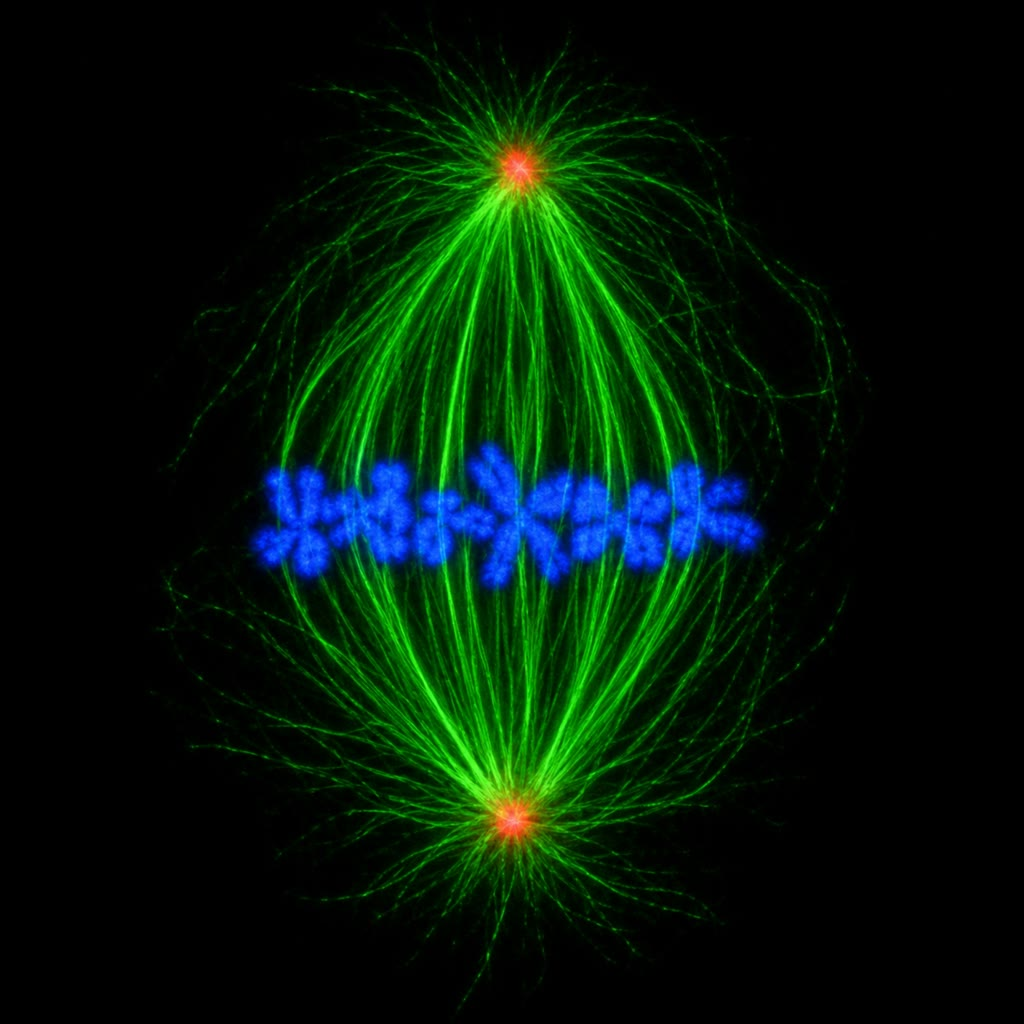
\includegraphics[width=0.36\linewidth]{images/book5/ai/b5-10-mitotic-spindle.jpg}\hspace{0.04\linewidth}
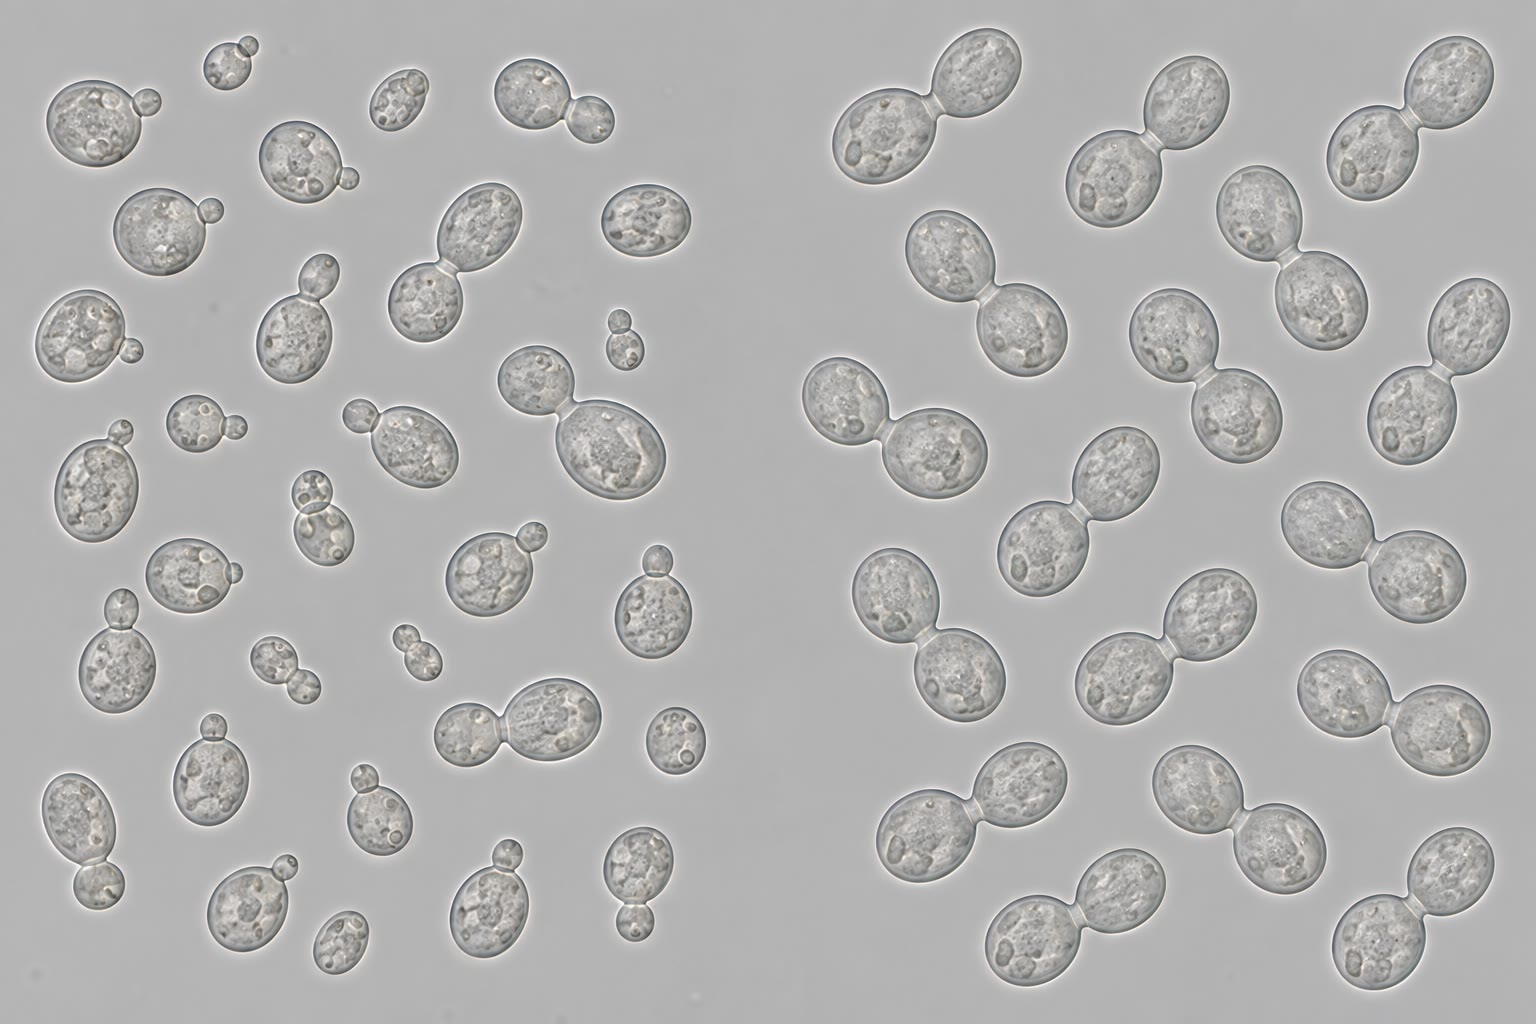
\includegraphics[width=0.54\linewidth]{images/book5/ai/b5-10-yeast-cdc-mutants.jpg}

{\small يسارًا: خلية في الطور الاستوائي --- أنيبيبات المغزل (بالأخضر) من
القطبين (بالأحمر)، والصبغيات (بالأزرق) مصطفة عند الصفيحة، وهي
اللحظة التي تقرر عندها \omterm{def:b3:cell-cycle-apoptosis:checkpoints}{نقطة تفتيش} المغزل. يمينًا: خميرة التبرعم،
النمط البري ببراعم من كل حجم (يسارًا) وطافر \emph{cdc}
توقفت فيه كل خلية عند الطور نفسه، ولكل منها برعم
بالحجم نفسه (يمينًا).}
\end{omfigure}

\section{الاستماتة}

\begin{definition}[الاستماتة]\label{def:b3:cell-cycle-apoptosis:apoptosis}
\index{استماتة}\index{نخر}\index{كاسباز}\index{فوسفاتيديل سيرين}
\emph{الاستماتة} موت خلوي مبرمج بتسلسل جوهري: فتنكمش
الخلية وتستدير، ويتكاثف صبغينها ويُقطع DNA فيها
بين الجسيمات النووية سلّمًا من القطع، وتتفكك النواة، و
ينتفط الغشاء في حويصلات محكمة، ويظهر الفوسفاتيديل سيرين على
الوجه الخارجي للغشاء إشارةَ ``كُلني''، وتُبتلع
الشظايا من الجيران أو البلعميات في غضون ساعة ---
بلا رشح، ومن ثم بلا التهاب. وتنفذها
\emph{الكاسبازات}، وهي بروتيازات سيستئينية تقطع بعد الأسبارتات، وتُصنع
خمائر غير فعالة: و\emph{الكاسبازات \omterm{def:b3:genetic-engineering:pcr}{البادئة}} (8 و9) تُنشَّط
بجمعها على منصة، وهي تشطر وتنشّط
\emph{الكاسبازات المنفِّذة} (3 و7)، التي تقطع عدة مئات من
الركائز --- اللامينات، والهيكل الخلوي، ومثبط
النوكلياز القاطع لجزيء DNA، والإنزيم الذي يبقي الفوسفاتيديل سيرين في الداخل.
أما \emph{النخر} فموت بالأذية: إذ تنتفخ الخلية، و
تنفجر، وتسكب محتوياتها وتثير الالتهاب. وقد سمّى الاستماتةَ
ووصف شكلَها كير وويلي وكوري (1972)؛
ووُجدت مورّثاتها في دودة.
\end{definition}

\begin{proof}[شواهد]
كل خنثى من \emph{Caenorhabditis elegans} تصنع $1090$ خلية
جسدية، يموت منها $131$ الخلايا نفسها، كل واحدة في زمن وموضع محددين.
وعزل هورفيتز وزملاؤه (في الثمانينيات) طافرات نجت فيها:
و\emph{ced-3} و\emph{ced-4} كانتا لازمتين لكل موت، وفي
غيابهما عاشت الخلايا $131$ وتمايزت؛ و\emph{ced-9}
كانت تحمي --- ففقدها يقتل خلايا كان ينبغي أن تعيش، وفرطُ نشاطها
ينقذ خلايا كان ينبغي أن تموت؛ و\emph{egl-1} كانت
لازمة لموتات بعينها. وتبيّن أن CED-3 \omterm{def:b3:cell-cycle-apoptosis:apoptosis}{كاسباز}، وCED-4 منصته
المنشّطة (وهي Apaf-1 في البشر)، وCED-9 بروتين من \omterm{def:b3:cell-cycle-apoptosis:pathways}{أسرة Bcl-2}، وEGL-1
بروتين من صنف BH3 وحده: أي المسلك البشري، مورّثةً مورّثة. وكانت
مورّثة \emph{BCL2} البشرية قد وُجدت عند انتقال صبغي في
اللمفومة الجريبية، وهي سرطان خلايا تخفق في الموت.
\end{proof}

\begin{definition}[المسلكان]\label{def:b3:cell-cycle-apoptosis:pathways}
\index{مسلك جوهري}\index{مسلك خارجي}\index{أسرة Bcl-2}\index{سيتوكروم c}\index{جسيم الاستماتة}\index{مستقبل الموت}
المسلك \emph{الجوهري} (المتقدري) يجمع حالة الخلية
الداخلية. ولدى \emph{أسرة Bcl-2} ثلاثة أصناف: حرّاس
(Bcl-2، وBcl-xL، وMcl-1) يجلسون على الغشاء المتقدري الخارجي و
يبقونه محكمًا؛ ومنفّذات (Bax، وBak) تتألف، متى نُشّطت،
مسامَّ في ذلك الغشاء؛ ومستشعرات من \emph{صنف BH3 وحده} (Bim، وBid،
وPuma، وNoxa، وBad)، يحرّض أو ينشّط كلًا منها أذًى بعينه ---
أذية DNA عبر p53 (Puma وNoxa)، وسحب عامل النمو (Bim،
وBad)، والانفصال، والبروتينات غير المطوية --- فترتبط بالحرّاس و
تحرر المنفّذات أو تنشّطها. ومتى غلبت المنفّذات، نفذ الغشاء الخارجي، و
رشح \emph{السيتوكروم~c} إلى العصارة، فارتبط
بالبروتين Apaf-1 وكوّن \emph{جسيم \omterm{def:b3:cell-cycle-apoptosis:apoptosis}{الاستماتة}}، الذي ينشّط \omterm{def:b3:cell-cycle-apoptosis:apoptosis}{الكاسباز}~9. أما
المسلك \emph{الخارجي} فيبدأ من الخارج: إذ تستقدم \emph{مستقبلات الموت} (Fas،
ومستقبل TNF، ومستقبلات TRAIL)، حين ترتبط بها روابطها على لمفاوية
قاتلة أو خلية جارة فتتعنقد، وسائطَ وتنشّط
\omterm{def:b3:cell-cycle-apoptosis:apoptosis}{الكاسباز}~8، الذي يشطر \omterm{def:b3:cell-cycle-apoptosis:apoptosis}{الكاسباز}~3 مباشرةً، ويفتح أيضًا عبر Bid
الطريقَ المتقدري. ويلتقي المسلكان عند
الكاسبازات المنفِّذة، وتضبط بروتينات مثبطة (IAP، وFLIP)
العتبة على الطريق.
\end{definition}

\begin{omfigure}
\begin{tikzpicture}[every node/.style={font=\scriptsize}, >=stealth]
  % extrinsic
  \node[draw, thick, rounded corners, fill=omProp!25, align=center] (lig) at (0,4.2) {رابطة موت على خلية قاتلة\\(FasL، وTNF، وTRAIL)};
  \node[draw, thick, rounded corners, fill=omProp!25, align=center] (rec) at (0,2.8) {تتعنقد مستقبلات الموت؛\\وتستقدم الوسائط الكاسباز-8};
  \node[draw, thick, rounded corners, fill=omThm!20] (c8) at (0,1.5) {الكاسباز-8 فعال};
  % intrinsic
  \node[draw, thick, rounded corners, fill=omDef!20, align=center] (insult) at (7.2,4.2) {أذية DNA (p53)، وفقد عامل النمو،\\والانفصال، والبروتينات غير المطوية};
  \node[draw, thick, rounded corners, fill=omDef!20, align=center] (bh3) at (7.2,3.0) {مستشعرات BH3 وحده (Puma، وBim، وBid)\\تعادل Bcl-2، وتنشّط Bax/Bak};
  \node[draw, thick, rounded corners, fill=omDef!20, align=center] (mito) at (7.2,1.7) {ينفتح الغشاء المتقدري الخارجي:\\يخرج السيتوكروم $c$، ويتكوّن جسيم الاستماتة};
  \node[draw, thick, rounded corners, fill=omThm!20] (c9) at (7.2,0.5) {الكاسباز-9 فعال};
  % convergence
  \node[draw, thick, rounded corners, fill=omThm!35, align=center] (c3) at (3.6,-0.8) {الكاسبازان المنفِّذان 3 و7:\\قطع مئات الركائز};
  \node[draw, thick, rounded corners, fill=gray!15, align=center] (out) at (3.6,-2.3) {تكاثف الصبغين، وتسلّم DNA، والتنفط،\\وكشف الفوسفاتيديل سيرين، والابتلاع};
  \draw[->, thick] (lig) -- (rec); \draw[->, thick] (rec) -- (c8); \draw[->, thick] (c8) -- (c3);
  \draw[->, thick] (insult) -- (bh3); \draw[->, thick] (bh3) -- (mito); \draw[->, thick] (mito) -- (c9); \draw[->, thick] (c9) -- (c3);
  \draw[->, thick] (c3) -- (out);
  \draw[->, thick, dashed] (c8) -- (bh3) node[pos=0.55, below, sloped] {شطر Bid: يلتقي الطريقان};
  \node[left, omThm, align=right] at (-2.3,1.5) {المسلك\\الخارجي}; \node[right, omDef, align=left] at (10.4,1.7) {المسلك\\الجوهري};
  \node[right, font=\tiny, align=left] at (8.6,0.5) {تثبّط IAP هنا؛\\ويحرس Bcl-2 أعلاه};
\end{tikzpicture}

{\small الطريقان إلى الكاسبازات المنفِّذة. من الخارج إلى الداخل، ينشّط \omterm{def:b3:cell-cycle-apoptosis:pathways}{مستقبل
الموت} الكاسبازَ-8؛ ومن الداخل إلى الخارج، تزن \omterm{def:b3:cell-cycle-apoptosis:pathways}{أسرة Bcl-2}
حالةَ الخلية، ومتى غلبت المنفّذات أطلقت المتقدرة
السيتوكروم~$c$ ونُشّط الكاسباز-9. ويلتقي الطريقان عند الكاسباز-3.}
\end{omfigure}

\begin{proposition}[نقطة اللاعودة]\label{prop:b3:cell-cycle-apoptosis:mompt}
\index{نفاذية الغشاء المتقدري الخارجي}
نفاذُ الغشاء المتقدري الخارجي مفاجئ
--- إذ تنفتح متقدرات الخلية كلها في نحو خمس دقائق،
بعد ساعات من التداول --- وتامّ: فمتى صار السيتوكروم~$c$
في العصارة، تبع تنشيطُ الكاسبازات في دقائق ولم يمكن
إبطاله بإزالة المنبّه. وسمتان تجعلانه مفتاحًا. فمسام
Bax/Bak يتكوّن بالتألف، فيرتفع معدله ارتفاعًا حادًا مع
كمية المنفّذ المنشَّط؛ والحرّاس والمستشعرات يرتبط بعضها ببعض
بألفة عالية، حتى إنه حتى عتبة معينة يكون كل مستشعر
معادَلًا وبعدها يكون كل مستشعر إضافي حرًا --- أي معايرة،
كمحلول منظم يُستنفد. فالخلية لا تموت
تدريجيًا؛ بل تتراكم فيها بروتينات BH3 وحده حتى تُتجاوز عتبة،
فتموت دفعةً واحدة. والأدوية التي تحاكي بروتينات BH3
(الفينيتوكلاكس، الذي يشغل Bcl-2) تدفع الخلايا ``المهيّأة'' ---
أي التي هي قرب العتبة سلفًا، كما هي كثير من خلايا الابيضاض --- فوقها،
مع إعفاء التي ليست كذلك.
\end{proposition}

\begin{omfigure}
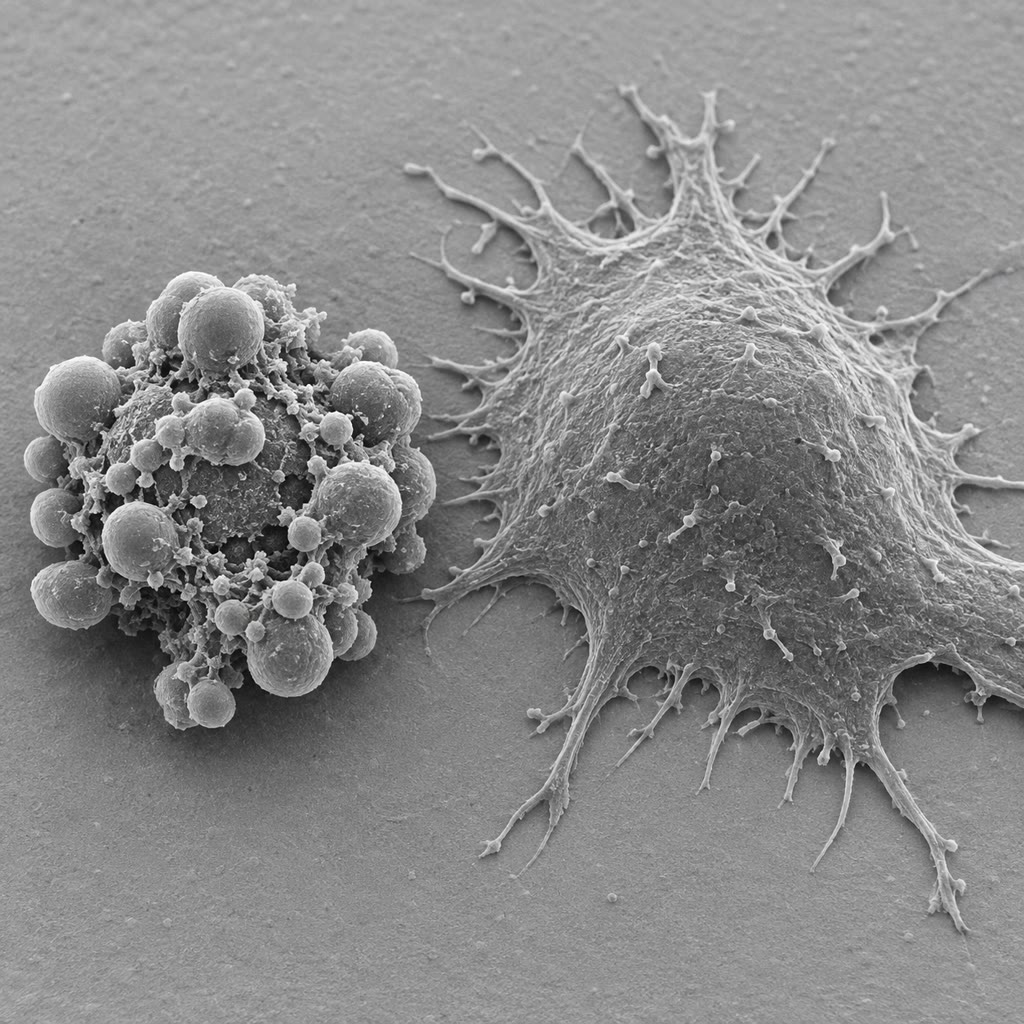
\includegraphics[width=0.40\linewidth]{images/book5/ai/b5-10-apoptotic-cell.jpg}

{\small خلية مستميتة بجانب أخرى سليمة في المجهر الإلكتروني
الماسح: منكمشة، وسطحها مقسّم إلى نفطات محكمة ستُبتلع
بلا أثر من التهاب.}
\end{omfigure}

\begin{example}[موتات تبني جسدًا]\label{ex:b3:cell-cycle-apoptosis:development}
تُنحت الأصابع من مجذاف \omterm{def:b3:cell-cycle-apoptosis:apoptosis}{باستماتة} الخلايا
بينها؛ وفي البط تعيش الخلايا نفسها ويبقى الغشاء بينها.
ويُمتصّ ذيل الشرغوف عند التحول على إشارة من
هرمون الدرق. ويموت نحو نصف العصبونات المنتَجة في الجملة
العصبية عند الفقاريات قبل الولادة، وهي التي تخفق في تلقي ما يكفي
من العامل المغذي من أهدافها --- أي منافسة توائم
عدد العصبونات مع حجم الحقل الذي تخدمه. ويموت خمسة وتسعون في
المئة من الخلايا التائية المصنوعة في التوتة هناك، إذ يُنتقى بعضها للإقصاء لأنها
لا تتعرف شيئًا أو تتعرف الذات (\cref{ch:b3:adaptive-immunity}).
وكل يوم تنبذ ظهارة الأمعاء أقدم خلاياها عند
قمم الزغابات، وينبذ الجلد خلاياه القرنية، وينبذ الدم عدلاته الهرمة
بعد عمر يوم: \omterm{def:b3:cell-cycle-apoptosis:apoptosis}{فالاستماتة} هي القاعدة، وحجم النسيج
هو الفرق بين معدلين كبيرين.
\end{example}

\section{مخارج أخرى، والإخفاق في الخروج}

\begin{definition}[النخر المنظَّم والشيخوخة الخلوية]\label{def:b3:cell-cycle-apoptosis:other}
\index{نخر مبرمج}\index{موت التهابي}\index{شيخوخة خلوية}
للخلايا موتات مبرمجة أخرى، كلها التهابية حيث تكون \omterm{def:b3:cell-cycle-apoptosis:apoptosis}{الاستماتة}
صامتة. و\emph{\omterm{def:b3:cell-cycle-apoptosis:apoptosis}{النخر} المبرمج}، الذي تطلقه مستقبلات الموت حين
يُحجب الكاسباز-8 (كما تحجبه بعض الفيروسات)، يجمّع الكيناز
RIPK3 مع MLKL، الذي يثقب الغشاء الهيولي. و\emph{الموت الالتهابي}،
في البلعميات المصابة، ينفذه الكاسباز-1 في الجسيم الالتهابي
(\cref{ch:b3:innate-immunity})، الذي يشطر الغازديرمين إلى
مكوّن مسام ويطلق الإنترلوكين-1. و\emph{الموت الحديدي} موت
بأكسدة الدهون المعتمدة على الحديد. وتستطيع الخلية أيضًا أن تكفّ عن الانقسام
من غير أن تموت: و\emph{الشيخوخة الخلوية} توقف دائم، يفرضه p16
وp21 بعد تآكل القسيمات الطرفية (\cref{ch:b3:stem-cells})، أو أذية DNA
المستمرة أو تنشيط مورّثة ورمية، تبقى فيه الخلية نشطة استقلابيًا
وتفرز عوامل التهابية. والشيخوخة الخلوية تزيل الخلايا المتأذية
من مخزون الانقسام --- فهي كابح ورم --- وتتراكم
مع العمر، حيث تسهم إفرازاتها في تنكس
الأنسجة؛ وتنظيف الخلايا الشائخة في الفئران يطيل الحياة الصحية.
\end{definition}

\begin{remark}[القليل جدًا والكثير جدًا]\label{rem:b3:cell-cycle-apoptosis:disease}
أمراض هذين البرنامجين أمراض جرعة. فالموت القليل جدًا:
سرطان، ترتفع فيه عتبة \omterm{def:b3:cell-cycle-apoptosis:apoptosis}{الاستماتة} بفرط التعبير عن Bcl-2
أو بفقد p53، فتنجو الخلايا ذات الجينومات المتأذية
لتراكم مزيدًا من الأذية؛ ومناعة ذاتية، حين تبقى اللمفاويات التي
كان ينبغي أن تموت في الانتقاء. والموت الكثير جدًا: فقدُ الخلايا التائية في
خمج HIV، وموتُ عصبونات شبه ظل السكتة \omterm{def:b3:cell-cycle-apoptosis:apoptosis}{بالاستماتة} بعد ساعات
من الإقفار (وهو نافذة للعلاج)، \omterm{def:b3:cell-cycle-apoptosis:apoptosis}{والاستماتة} البطيئة
للعصبونات في أمراض التنكس العصبي، وفقدُ الخلايا القلبية بعد
احتشاء. ومعالجة السرطان في معظمها إحداثٌ متعمد
\omterm{def:b3:cell-cycle-apoptosis:apoptosis}{للاستماتة} في خلايا عتباتها أدنى من عتبات جاراتها،
والأدوية التي تستهدف Bcl-2 وCdk4/6 هي أول ما صُمم
من خرائط هذا الفصل.
\end{remark}

\section{تمارين}

\begin{exercise}[$\star$]\label{exo:b3:cell-cycle-apoptosis:1}
عدّد أطوار الدورة الأربعة، وزوج السيكلين--CDK الذي يقود
كل انتقال، وليغاز اليوبيكويتين الذي ينهي الانقسام الفتيلي.
\end{exercise}

\begin{exercise}[$\star$]\label{exo:b3:cell-cycle-apoptosis:2}
بماذا أسهم كل من هارتويل ونيرس وهانت في اكتشاف
المحرّك، وفي أي كائن؟
\end{exercise}

\begin{exercise}[$\star$]\label{exo:b3:cell-cycle-apoptosis:3}
سمِّ نقاط التفتيش الثلاث، والشرط الذي تختبره كل منها، و
الهدف الجزيئي الذي تعمل عليه كل منها.
\end{exercise}

\begin{exercise}[$\star$]\label{exo:b3:cell-cycle-apoptosis:4}
ميّز \omterm{def:b3:cell-cycle-apoptosis:apoptosis}{الاستماتة} من \omterm{def:b3:cell-cycle-apoptosis:apoptosis}{النخر} في خمس سمات، وسمِّ
صنف الإنزيمات الذي ينفذ \omterm{def:b3:cell-cycle-apoptosis:apoptosis}{الاستماتة}.
\end{exercise}

\begin{exercise}[$\star\star$]\label{exo:b3:cell-cycle-apoptosis:5}
في مستخلص بيضة ضفدع يُركَّب \omterm{def:b3:cell-cycle-apoptosis:cdk}{السيكلين} B بمعدل $k_{s} = 1$ وحدة في
الدقيقة؛ وعتبة الانقسام الفتيلي $C_{2} = 30$ وحدة، وعتبة الخروج
$C_{1} = 5$، ويُحلَّل \omterm{def:b3:cell-cycle-apoptosis:cdk}{السيكلين} في الانقسام بعمر نصف قدره
\qty{2}{min}. قدّر دور التذبذب ونسبة
الدورة التي تُقضى في الانقسام الفتيلي.
\end{exercise}

\begin{exercise}[$\star\star$]\label{exo:b3:cell-cycle-apoptosis:6}
تنبأ بسلوك خلية (أ) تعبّر عن \omterm{def:b3:cell-cycle-apoptosis:cdk}{سيكلين} B غير قابل
للتحلل، و(ب) ينقصها Wee1، و(ج) ينقصها Cdc25، و(د) تعبّر عن Cdk1
لا يستطيع Wee1 فسفرته، بدلالة مذبذب
\cref{thm:b3:cell-cycle-apoptosis:oscillator}.
\end{exercise}

\begin{exercise}[$\star\star$]\label{exo:b3:cell-cycle-apoptosis:7}
دمج راو وجونسون يصل خلية في G1 بخلية في الطور S؛ وآخر
يصل خلية في G2 بخلية في الطور S. تنبأ بما تفعله كل نواة و
فسّر ذلك بالترخيص وبمستويات CDK.
\end{exercise}

\begin{exercise}[$\star\star$]\label{exo:b3:cell-cycle-apoptosis:8}
فسّر لماذا يستطيع قسيم مركزي واحد غير مرتبط أن يوقف الطور الانفصالي
في الخلية كلها، وتنبأ بمصير خلية حُذف فيها
Mad2.
\end{exercise}

\begin{exercise}[$\star\star$]\label{exo:b3:cell-cycle-apoptosis:9}
تنبأ بالنمط الظاهري لدودة ينقصها \emph{ced-9}؛ وينقصها
\emph{ced-3}؛ وينقصها كلاهما. وفسّر التفوق الوراثي بدلالة
المسلك.
\end{exercise}

\begin{exercise}[$\star\star\star$]\label{exo:b3:cell-cycle-apoptosis:10}
بيّن أن عروة تغذية راجعة سالبة واحدة بلا مفتاح ثنائي الاستقرار
--- \omterm{def:b3:cell-cycle-apoptosis:cdk}{سيكلين} يُركَّب بمعدل $k_{s}$، ويُحلَّل بمعدل $k_{d}AC$ حيث $A$
متناسبة ببساطة مع $C$ --- لها حالة مستقرة ثابتة ولا
تتذبذب. فماذا يضيف المنحني الذي على شكل S، وماذا كان تأخيرٌ
ليضيف بدلًا منه؟
\end{exercise}

\begin{exercise}[$\star\star\star$]\label{exo:b3:cell-cycle-apoptosis:11}
لخلية $N$ جزيء من الحارس Bcl-2 وتتلقى مستشعرات من صنف BH3
وحده بمعدل $r$ في الساعة بعد منبّه ضار، ويربط كل مستشعر
حارسًا واحدًا. فسّر لماذا تموت الخلية عند الزمن $N/r$ تقريبًا
أيًا كانت شدة المنبّه فوق ذلك، ولماذا يكون الموت مفاجئًا،
وماذا يفعل الفينيتوكلاكس بالزمن.
\end{exercise}

\begin{exercise}[$\star\star\star$]\label{exo:b3:cell-cycle-apoptosis:12}
تحمل اللمفومة الجريبية انتقالًا صبغيًا يفرط في التعبير عن
\emph{BCL2}؛ وخلاياها تنقسم ببطء. ويحمل الورم الأرومي الشبكي فقدَ
\emph{RB}؛ وخلاياه تنقسم سريعًا. فسّر كيف تنتج كل آفة منفردة
ورمًا، ولماذا يكون الأول وديعًا والثاني عدوانيًا،
وماذا يقول كل منهما عن برنامجي هذا الفصل.
\end{exercise}

\section{مسألة: حياة ظهارة وموتها}

\begin{problem}[{مسألة نهاية الأسبوع --- بطانة الأمعاء مجددةً خليةً
خليةً، والدورة موقوتةً من مذبذب السيكلين، وأخطاء
نقطة تفتيش معدودة على مستوى الجسم، والتخلص الاستماتي من
مئة مليار خلية في اليوم موزونًا، وتنتهي إلى دور الدورة، و
الخلايا المختلة الصيغة المنتَجة في اليوم والكتلة التي يعيد الجسم
تدويرها بالاستماتة}]
\label{pb:b3:cell-cycle-apoptosis:1}
معطيات: في الأمعاء الدقيقة $10^{7}$ خبيئة، تجدد كل منها زغابة
من \num{3500} خلية كل $5$ أيام؛ وتحوي كل خبيئة نحو $22$ خلية
جذعية تنقسم مرة في اليوم، وتنقسم ذريتها $5$ مرات أخرى قبل
أن تتمايز. والمذبذب: $k_{s} = 2$ وحدة \omterm{def:b3:cell-cycle-apoptosis:cdk}{سيكلين} في الساعة، و
$C_{2} = 40$ وحدة، و$C_{1} = 8$، وعمر نصف \omterm{def:b3:cell-cycle-apoptosis:cdk}{السيكلين} الانقسامي
\qty{10}{min}. \omterm{def:b3:cell-cycle-apoptosis:checkpoints}{ونقطة التفتيش}: من دون \omterm{def:b3:cell-cycle-apoptosis:checkpoints}{نقطة تفتيش} المغزل يخطئ انقسام
من كل $50$ في فرز صبغي؛ ومعها واحد من \num{50000}.
ويستبدل الجسم $10^{11}$ خلية في اليوم كتلة كل منها \qty{1}{ng}، والبروتين
\qty{20}{\%} من الكتلة؛ ويصفّي البلعمي خلية مستميتة واحدة في
\qty{1}{h}.

\medskip
\noindent\textbf{الجزء الأول --- التجديد.}
\begin{enumerate}
  \item كم خلية تنبذ الأمعاء الدقيقة في اليوم، وكم في
        الثانية؟
  \item كم خلية تنتج الخبيئة الواحدة في اليوم؟ وللتحقق: $22$
        انقسامًا جذعيًا في اليوم، وكل بنت ملتزمة تنقسم $5$ مرات
        أخرى.
  \item إذا انقسمت خلية جذعية مرة في اليوم على مدى عمر قدره $80$ سنة،
        فكم انقسامًا؟ وبمعدل طفرة قدره $0.6$ لكل جينوم في
        الانقسام (\cref{ch:b3:dna-repair})، كم طفرة
        تتراكم فيها؟
  \item تنقسم خلايا العبور كل \qty{12}{h}. فلماذا يستطيع النسيج
        أن يتحمل انقسامات عبور سريعة قصيرة العمر لكنه يبقي الخلية
        الجذعية بطيئة؟
  \item جرعة إشعاع تقتل خلايا العبور المنقسمة كلها لكنها
        تعفي الخلايا الجذعية، التي تستأنف في غضون يوم. فكم
        يمضي قبل أن تصير الزغابة، بلا تجديد، عاريةً، وكم يلزم
        لإعادة بنائها؟ ولماذا تكون الأمعاء ضحية باكرة للإشعاع؟
  \item في القولون يكون النبذ في الأعلى \omterm{def:b3:cell-cycle-apoptosis:apoptosis}{بالاستماتة} (أي موت الانفصال،
        وهو الموت عند الانفصال). فلماذا يكون هذا نمط الموت الصحيح
        لخلية على تماس مع بكتيريا الأمعاء؟
\end{enumerate}

\medskip
\noindent\textbf{الجزء الثاني --- الساعة.}
\begin{enumerate}[resume]
  \item من معطيات المذبذب، كم يستغرق \omterm{def:b3:cell-cycle-apoptosis:cdk}{السيكلين} ليرتفع
        من $C_{1}$ إلى $C_{2}$؟
  \item وكم يستغرق التحلل الانقسامي ليهبط به من $C_{2}$
        عائدًا إلى $C_{1}$؟
  \item دور المذبذب العاري، ونسبة الدور التي يُقضى فيها
        مع Cdk1 فعال.
  \item تدور خلايا العبور في الخبيئة في \qty{12}{h}، والخلايا الجذعية
        في \qty{24}{h}، وبيضة الضفدع في \qty{30}{min}. فأي وسائط
        النموذج يختلف، وما الذي يوفر
        الفرق في خلية جسدية؟
  \item خلية متوقفة عند \omterm{def:b3:cell-cycle-apoptosis:checkpoints}{نقطة تفتيش} G2/M بسبب أذية DNA تظل
        تصنع \omterm{def:b3:cell-cycle-apoptosis:cdk}{السيكلين} B. فأين تقع في مستوي الطور، وما الذي
        يمسكها هناك؟ وماذا يحدث حين يُصلَح الأذى؟
  \item دواء يثبط APC/C. صِف مصير خلية تدخل
        الانقسام الفتيلي بحضوره.
\end{enumerate}

\medskip
\noindent\textbf{الجزء الثالث --- الأخطاء.}
\begin{enumerate}[resume]
  \item كم انقسامًا في اليوم ينفذ الجسم ليستبدل
        $10^{11}$ خلية؟
  \item كم بنتًا مختلة الصيغة في اليوم مع \omterm{def:b3:cell-cycle-apoptosis:checkpoints}{نقطة التفتيش}، و
        من دونها؟
  \item معظم الخلايا المختلة الصيغة تموت أو تتوقف (إذ يستجيب p53
        لسوء الفرز). فإذا نجا \qty{1}{\%} وانقسم، فكم خلية
        مختلة الصيغة منقسمة ينتج جسم سليم نقطةَ التفتيش
        في اليوم، وكم على مدى عمر؟
  \item ورم من $10^{9}$ خلية فقد \omterm{def:b3:cell-cycle-apoptosis:checkpoints}{نقطة التفتيش} وفقد p53.
        فكم سوء فرز ينفذ في اليوم، ولماذا يجعله
        ذلك يتطور سريعًا؟
  \item فسّر لماذا يكون الفقد التام \omterm{def:b3:cell-cycle-apoptosis:checkpoints}{لنقطة تفتيش} المغزل
        مميتًا لجنين مع أن الفقد الجزئي يعزز السرطان.
  \item تنشأ متلازمة داون من سوء فرز في الانقسام المنصّف لا
        الفتيلي. فسّر لماذا يصيب خطأ في خلية واحدة هناك كل
        خلية عند الطفل، بينما يصيب خطأ فتيلي واحد سلالة واحدة.
\end{enumerate}

\medskip
\noindent\textbf{الجزء الرابع --- التخلص.}
\begin{enumerate}[resume]
  \item ما كتلة الخلايا التي يتخلص منها الجسم \omterm{def:b3:cell-cycle-apoptosis:apoptosis}{بالاستماتة} في
        اليوم، وفي السنة؟ قارنها بكتلة الجسم.
  \item كم من البروتين ذلك في اليوم؟ قارنه بمدخول
        غذائي قدره \qty{70}{g}: فما نسبة إعادة تدوير الخلايا الميتة
        من دوران بروتين الجسم؟
  \item كم بلعميًا، يعمل باستمرار، يلزم
        لتصفية موتى اليوم؟ وفي الجسم نحو $10^{11}$
        بلعمي: فما نسبة وقتها؟
  \item لماذا يجب أن تُزال الجثة قبل أن تتحلل، وما الذي
        يشير إلى ``كُلني''؟
  \item مريض يفرط في التعبير عن Bcl-2 في خلاياه البائية. فأي مسلك
        محجوب، وهل ما يزال \omterm{def:b3:cell-cycle-apoptosis:pathways}{المسلك الخارجي} يعمل، ولماذا تكون
        النتيجة لمفومة بطيئة النمو لا سريعته؟
  \item عصبونات شبه ظل السكتة تموت \omterm{def:b3:cell-cycle-apoptosis:apoptosis}{بالاستماتة} بعد ست إلى
        أربع وعشرين ساعة من الإصابة، وعصبونات اللب \omterm{def:b3:cell-cycle-apoptosis:apoptosis}{بالنخر}
        في دقائق. فلماذا يتيح الأول نافذة
        للعلاج ولا يتيحها الثاني؟
  \item لخّص: دور المذبذب العاري (السؤال~9)، و
        الخلايا المختلة الصيغة المنقسمة في اليوم في جسم سليم
        (السؤال~15)، والكتلة المعاد تدويرها \omterm{def:b3:cell-cycle-apoptosis:apoptosis}{بالاستماتة} في اليوم
        (السؤال~19).
\end{enumerate}
\end{problem}
